Взятая за основу схема БПЛА-ЦАГИ выполнена по схеме ``бесхвостка''. Габаритные размеры БПЛА: 
\begin{itemize}
\item размах крыльев: $\approx37\text{м}$
\item высота фюзеляжа: 1.7м
\item длина фюзеляжа: 7м
\end{itemize}


\begin{figure}[H]
\centering
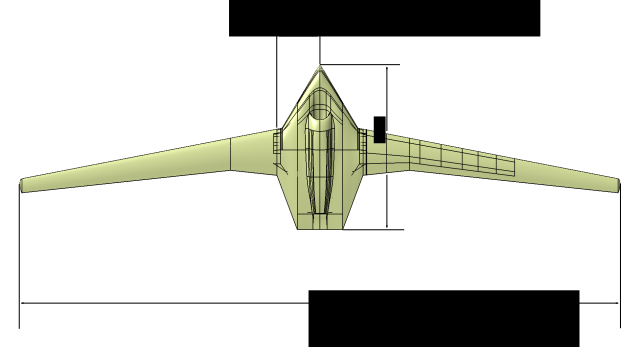
\includegraphics[width=0.8\textwidth]{BPS_Catia_Top}
\caption{Вид сверху}
\label{fig:BPS_Catia_Top}
\end{figure}

Как видно из Рис.\ref{fig:BPS_Catia_Top}, в данной схеме используются крылья большого удлинения. На рисунке \ref{fig:BPS_Catia_WithoutSkin} можно видеть, как крыло интегрировано с фюзеляжем для лучшей передачи нагрузок с крыла на фюзеляжную часть центроплана.


\begin{figure}[H]
\centering
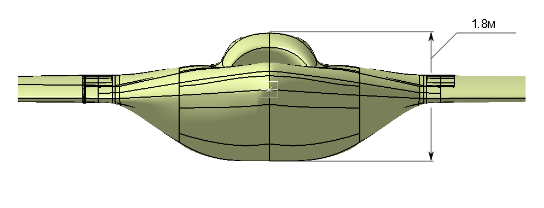
\includegraphics[width=0.8\textwidth]{BPS_Catia_Front}
\caption{Вид фюзеляжа спереди}
\label{fig:BPS_Catia_Front}
\end{figure}




\begin{figure}[H]
\centering
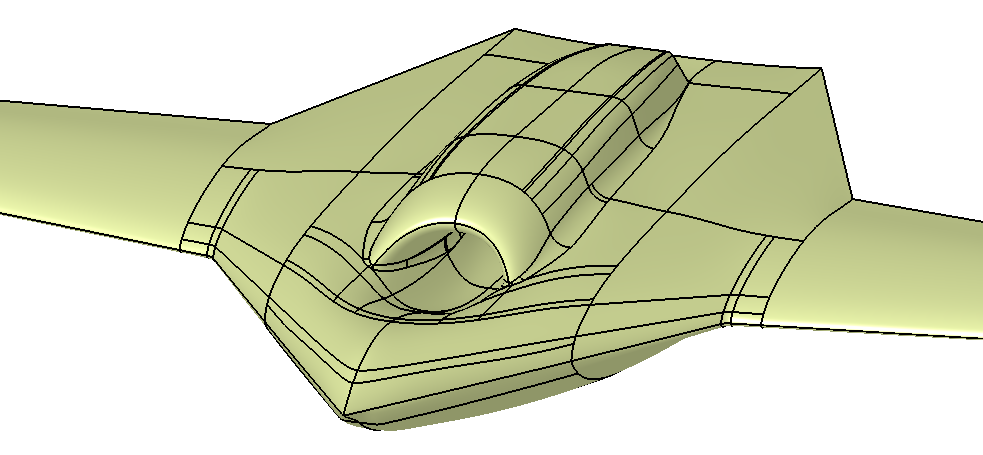
\includegraphics[width=0.8\textwidth]{BPS_Catia}
\caption{Вид фюзеляжа в изометрии}
\label{fig:BPS_Catia}
\end{figure}

\begin{figure}[H]
\centering
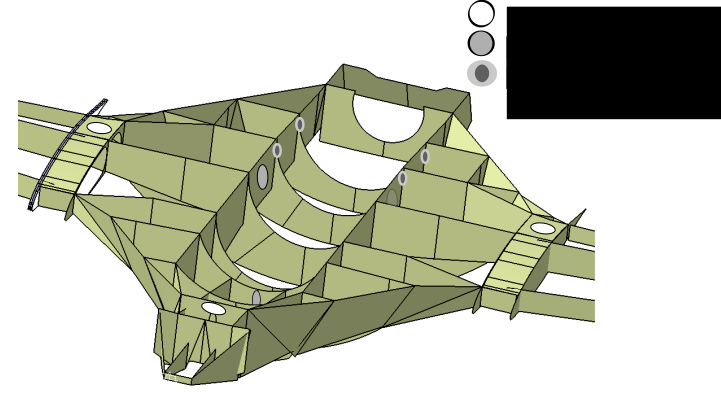
\includegraphics[width=0.8\textwidth]{BPS_Catia_WithoutSkin}
\caption{Вид фюзеляжа со снятой обшивкой}
\label{fig:BPS_Catia_WithoutSkin}
\end{figure}

Также на Рис. \ref{fig:BPS_Catia}, \ref{fig:BPS_Catia_WithoutSkin} видно, что двигатель с воздухозаборником утоплены в конструкцию. Это позволяет значительно улучшить малозаметность и аэродинамическое качество самолета (ссылка на отчет), но приводит к необходимости использовать искривленный центроплан. 

В данной схеме используется только горизонтальное оперение: руль высоты. Механизация крыла состоит из расщепляющихся элеронов на концах крыльев, обычных элеронов и интерцепторов. В качестве тяги используется один реактивный двигатель, установленный в канале. Места креплений стоек и замков шасси, расположение двигателя и узлов его крепления показаны на Рис. \ref{fig:BPS_Catia_Top_WithoutSkin}. 


\begin{figure}[H]
\centering
\def\svgwidth{0.9\textwidth}
\input{figures/BPS_Catia_Top_WithoutSkin.pdf_tex}
\caption{Вид сверху без обшивки с указанием узлов крепления шасси и двигателя}
\label{fig:BPS_Catia_Top_WithoutSkin}
\end{figure}

Отсеки фюзеляжа делятся на несколько групп по назначению. Распределение отсеков фюзеляжа по назначению представлено на Рис.\ref{fig:BPS_Catia_Top_PartRoles}. 


\begin{figure}[H]
\centering
\def\svgwidth{0.9\textwidth}
\input{figures/BPS_Catia_Top_PartRoles.pdf_tex}
\caption{Вид сверху с обозначением роли отсеков}
\label{fig:BPS_Catia_Top_PartRoles}
\end{figure}




Пока кратко: Крыло большого удлинения интегрировано с фюзеляжем. Двигатель утоплен в конструкцию, подвод воздухозаборника, сопло над горизонтальным оперением. В передней части фюзеляжа расположены отсеки с БРЭО, отсеки с топливом, отсек под переднее шасси. 
В задней части фюзеляжа пара отсеков под топливо, отсеки под БРЭО, шассийные отсеки, шасси крепится на стыке крыла с фюзеляжем. 







%Описываем полностью всю конструкцию. Показываем много разных картинок. 